\subsection{Dataset Utilizado}

Para el desarrollo del prototipo y la generación de texto se empleó el dataset \texttt{wikipedia.20220301.simple}, el cual corresponde a artículos de Wikipedia (edición Simple English) con fecha del 1 de marzo de 2022. Este dataset contiene aproximadamente 205,328 artículos.

El procesamiento realizado se resume en los siguientes pasos:

\begin{enumerate}
  \item Se extrajo únicamente el primer párrafo de cada artículo, como representación más concisa del contenido.
  \item Se filtraron los textos para  descartar aquellos que contuvieran caracteres distintos al alfabeto latino básico (es decir, se eliminaron caracteres como acentos inusuales, alfabetos no latinos, símbolos extraños o de otros idiomas).
  \item Se construyó un nuevo dataset que incluye únicamente los campos: id, title y text, ajustados a los criterios anteriores.
  \item Por ultimo, el dataset final se guardó localmente para ser utilizado durante el desarrollo del prototipo.
\end{enumerate}

Gracias a estos filtros, garantizamos que cada artículo utilizado contenga únicamente caracteres válidos del alfabeto latino, lo cual resulta esencial para asegurar que la generación de texto incluyendo la respuesta correcta usada para comparar con la del usuario sea consistente, legible y libre de interferencias lingüísticas irrelevantes.

Después de aplicar estos filtros, se obtuvo un total de  120,703 artículos, los cuales conforman la base para la generación de texto a partir de este dataset.


\subsection{Modelo para generación de texto}
El modelo que se utilizo para generar texto es el modelo pre-entrenado de GPT-2, el cual está basado en la arquitectura de transformadores (transformers). Esta arquitectura se caracteriza por el uso del mecanismo de atención self-attention, que permite que cada palabra del texto se relacione con todas las demás de la secuencia. GPT-2 es un modelo auto-regresivo, lo que significa que genera texto palabra por palabra, prediciendo la siguiente palabra dado el contexto anterior. La clase implementa el patrón de diseño Singleton, el cual asegura que solo exista una única instancia activa del modelo en memoria durante la ejecución del programa.

\newpage
\subsubsection{Parámetros de Generación}
La clase utiliza el método pipeline de Hugging Face para configurar la generación de texto. Los principales parámetros usados son:

\begin{table}[H]
\centering
{\small
\begin{tabular}{|l|p{5cm}|p{5cm}|l|}
\hline
\textbf{Par\'ametro} & \textbf{Definici\'on} & \textbf{Efecto en la Generaci\'on} & \textbf{Valor} \\
\hline
\texttt{num\_beams} & Cantidad de caminos posibles que el modelo explora para encontrar el mejor resultado. & Mejora la calidad del texto al considerar varias opciones de generaci\'on al mismo tiempo. & 5 \\
\hline
\texttt{temperature} & Controla cu\'anta variedad puede tener el texto generado. & Un valor bajo hace el texto m\'as predecible; uno alto lo hace m\'as creativo y diverso. & 0.9 \\
\hline
\texttt{top\_k} & Limita la elecci\'on de palabras a las m\'as probables. & Ayuda a que el texto sea coherente al evitar palabras poco comunes o sin sentido. & 45 \\
\hline
\texttt{no\_repeat\_ngram\_size} & Evita que se repitan grupos de palabras del mismo tama\~no. & Hace que el texto se sienta m\'as natural al eliminar repeticiones innecesarias. & 3 \\
\hline
\end{tabular}
}
\caption{Par\'ametros de generaci\'on de texto en GPT-2}
\label{tab:parametros_gpt2}
\end{table}

\subsubsection{Procesamiento del Texto}

Por motivos de control y calidad del texto generado, el texto base (un articulo que este dentro del dataset ya procesado) es truncado a 70 caracteres, con el fin de adquirir un contexto mínimo sobre el cual generar texto. Ademas el texto generado pasa por una etapa de limpieza para garantizar un resultado coherente y legible:

\begin{enumerate}
    \item Se recorta el texto hasta el último signo de puntuación válido.
    \item Se eliminan caracteres no deseados mediante expresiones regulares.
    \item Se normalizan los espacios múltiples.
\end{enumerate}

\subsection{Modelos para generación de preguntas y respuestas}

Para el sistema de preguntas y respuestas se utilizaron dos modelos distintos, cada uno con un propósito específico. El modelo t5-large-generation-race-QuestionAnswer, basado en la arquitectura T5 y entrenado con el dataset RACE, se utilizó para la generación estructurada de preguntas y respuestas extractivas. Por otro lado, el modelo t5-large-generation-squad-QuestionAnswer, entrenado con el conjunto de datos SQuAD, se empleó para la generación estructurada de preguntas y respuestas abstractivas. Esta combinación permite ofrecer al usuario una experiencia más completa ya que debe de responder a preguntas cuya respuesta se encuentra explícitamente e implícitamente en el contenido dado, reforzando así tanto sus habilidades de comprensión como de interpretación.

\newpage
\subsubsection{Generaci\'on de preguntas}

Los dos modelos utilizados para la generaci\'on de preguntas y respuestas son basasados en la arquitectura T5 (Text-To-Text Transfer-Transformer). Esta arquitectura convierte todas las tareas de procesamiento de lenguaje natural en tareas de texto a texto, es decir, dado un texto de entrada, genera un texto de salida.
\\
\\
La clase \texttt{RaceModel} implementa el patr\'on de dise\~no Singleton para el modelo t5-large-generation-race-QuestionAnswer, el cual garantiza que solo exista una instancia activa del modelo en memoria durante la ejecuci\'on. Esto permite optimizar el uso de recursos, evitando la recarga del modelo cada vez que se desee generar una pregunta y su respectiva respuesta. De la misma manera la clase \texttt{SquadModel} implementa el patron singleton para el modelo t5-large-generation-squad-QuestionAnswer.

\subsubsection{Parámetros de Generación}

La generación de texto se realiza mediante el uso de la función pipeline de Hugging Face, que facilita la configuración de los modelos pre-entrenados. En el caso de ambos modelos, se configuraron los mismos parámetros que se describen en la \autoref {tab:parametros_gpt2} num beams = 5, temperature = 0.7, top k = 50 y no repeat ngram size = 2.

\subsubsection{Procesamiento de preguntas y respuestas}

Para asegurar la calidad del contenido generado, se realiza un proceso de limpieza. Esto incluye:

\begin{enumerate}
    \item Eliminación de caracteres no deseados mediante expresiones regulares.
    \item Recorte de espacios en blanco innecesarios y normalización.
\end{enumerate}

\subsection{Modelo para generación de respuestas incorrectas}

El modelo encargado de la generación de respuestas incorrectas se basa en una versión adaptada de T5 bajo el nombre t5-large-generation-race-Distractor. Este modelo fue configurado específicamente para generar opciones incorrectas plausibles a partir de una pregunta, una respuesta correcta y un contexto. Para su ejecución se carga mediante la clase  \texttt{DistractorModel} mas el uso del patrón singleton, lo que garantiza que sólo se mantenga una instancia activa en memoria, optimizando el uso de recursos.
\\
\\
Durante la generación de preguntas incorrectas, se configuraron los mismos parámetros que se describen en la \autoref {tab:parametros_gpt2} num beams=5, no repeat ngram size=2, temperature=0.9 y top k=50. La entrada al modelo se construye uniendo la pregunta, la respuesta correcta y el contexto, el cual es el texto generado por gpt2.

\newpage
\section{Flujo completo de generación de lecciones}

Para iniciar el flujo de generación de lecciones, se utiliza \texttt{Celery Beat}, un componente de Celery que permite programar tareas periódicas. En este caso, la tarea principal llamada \texttt{generate\_lessons} se ejecuta cada 30 minutos. Esto se define en la configuración mediante la clave \texttt{beat\_schedule}, especificando el uso del metodo \texttt{crontab(minute='\*/30')}.

\subsection{Inicialización de Workers}
Al iniciar cada proceso worker, se ejecuta la función \texttt{init pools}, la cual asigna una semilla de generación pseudoaleatoria distinta a cada uno, evitando así patrones repetitivos en la generación.
\\
\\
Esta estrategia es especialmente importante dado que Celery, por defecto, utiliza un pool prefork para la ejecución de tareas. El modo prefork consiste en la creación de múltiples procesos hijos a partir del proceso principal. Esto permite ejecutar tareas en paralelo aprovechando múltiples núcleos del CPU, pero también introduce ciertas consideraciones en la inicialización del estado interno de cada worker. Todos los procesos hijos heredan el estado de la memoria del proceso padre en el momento del \texttt{fork()}. Esto incluye el estado del generador de números pseudoaleatorios, lo que significa que sin una inicialización manual, todos los procesos hijos comenzarán con la misma semilla aleatoria y, por tanto, producirán secuencias idénticas de números pseudoaleatorios, lo cual afecta directamente a la generación de lecciones, generando las mismas lecciones por ciclo de trabajo.

\begin{figure}[H]
  \centering
  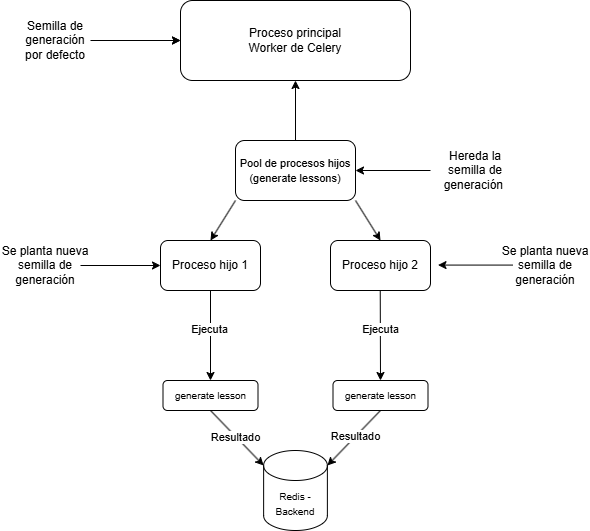
\includegraphics[width=0.7\linewidth]{Imagenes/diagrama de perfork.png}
  \caption{Diagrama de pool prefork en Celery}
  
  \label{fig:prefork}
\end{figure}

Para evitar este problema, como podemos ver en la figura~\ref{fig:prefork}, se utiliza la función \texttt{init pools} la cual se ejecuta justo después de que un proceso Worker ha sido inicializado y está listo para comenzar a ejecutar tareas. Dentro de init pools se realiza la lógica correspondiente para generar una semilla única con el método \texttt{random.seed()} realizando una combinación del PID (Process Identifier) del proceso (\texttt{os.getpid()}) y la marca de tiempo actual (\texttt{time.time()}). Con esto se garantiza que cada proceso tenga una secuencia única, evitando que se generen las mismas lecciones en cada ciclo.

\subsection{Tarea principal: generate lessons}
La tarea \texttt{generate lessons} es el punto de entrada del flujo. Esta tarea obtiene 6 muestras de texto desde el dataset previamente cargado usando la función \texttt{getDatasetText}.
\\
\\
A partir de estas muestras, se crean subtareas independientes mediante la tarea \texttt{generate\_lesson}, que son agrupadas y ejecutadas en paralelo. Una vez todas las lecciones han sido generadas, sus resultados se pasan a la tarea \texttt{save\_on\_dbs} para su almacenamiento.

\subsection{Generación de lecciones: generate\_lesson}
Cada subtarea de generación de lecciones sigue un proceso detallado:

\begin{enumerate}
\item Se genera un nuevo texto extendido a partir del texto de muestra usando un modelo basado en GPT-2 (\texttt{Gpt2Model}).
\item Si el texto generado tiene menos de 150 caracteres, se considera inválido y se re-intenta la tarea con una nueva muestra.
\item Se generan dos pares de pregunta-respuesta: uno usando el modelo RACE (\texttt{RaceModel}) y otro con el modelo SQuAD (\texttt{SquadModel}). Las preguntas y respuestas se separan usando el método \texttt{split\_qa}.
\item Para cada par de pregunta-respuesta, se genera una respuesta distractora utilizando el modelo \texttt{DistractorModel}. Si el distractor es igual a la respuesta, se re-intenta la generación.
\item Si todos los pasos son exitosos, se construye un objeto \texttt{LessonData} que agrupa el texto generado y las preguntas con sus respectivas respuestas y respuesta distractora.
\end{enumerate}

\subsection{Almacenamiento en bases de datos: save\_on\_dbs}
Una vez finalizadas todas las tareas de generación, los datos generados son almacenados en dos bases de datos:

\begin{itemize}
\item \textbf{Redis}: donde se guarda información ligera de cada lección en las estructuras definidas en la tabla \ref{table:EstructurasRedis}.
\item \textbf{PostgreSQL (NeonDB)}: donde se almacenan las preguntas y lecciones completas, manteniendo integridad referencial entre ellas.
\end{itemize}

Antes de realizar el guardado, se eliminan las lecciones anteriores con el propósito de que el usuario solo interactuare con las ultimas lecciones generadas.